 
%-------------------------------------------
% FILE:    training.tex
% AUTHOR:  Svea Hernandez, Jo Taylor, Bryan Hilbert
% DATE:    2013
%
% Master latex file for python training.
%
%-------------------------------------------


% Define style of document
\documentclass[12pt,letter]{book}% for A4 paper

% Include packages
\usepackage{float}
\usepackage{graphicx,palatino,palatcm}
\usepackage{amsmath,amssymb,amsfonts} % Typical maths resource packages
\usepackage{graphics}                 % Packages to allow inclusion of graphics
\usepackage{caption,topcapt}
\usepackage{rotating}
\usepackage{natbib}
\usepackage{wrapfig}
\usepackage{apjfonts}
\usepackage{amssymb}
\usepackage{multicol}
\usepackage{color}
\usepackage[colorlinks=true, urlcolor=blue]{hyperref}
\DeclareGraphicsRule{.tif}{png}{.png}{`convert #1 `dirname #1`/`basename #1 .tif`.png}

% Set the page layout
\setlength{\parindent}{0mm}      %sangria
\setlength{\textwidth}{161mm}
\setlength{\topmargin}{0mm}
\setlength{\textheight}{210mm}
\setlength{\oddsidemargin}{5mm}
\setlength{\evensidemargin}{-\oddsidemargin}
\setlength{\parskip}{3mm}     %espacio entre paragraphs
\linespread{1.0}   %determina el espacio entre lineas 1.6 = doble espacio

\usepackage{fancyhdr}
\pagestyle{fancy}
\renewcommand{\chaptermark}[1]%
   {\markboth{\uppercase{\thechapter.\ #1}}{}}
\renewcommand{\sectionmark}[1]%
   {\markright{\uppercase{\thesection.\ #1}}}
\newcommand{\helv}{%
   \fontfamily{phv}\fontseries{b}\fontsize{9}{11}\selectfont}
\lhead[\helv \thepage]{\helv \rightmark}
\rhead[\helv \leftmark]{\helv \thepage}
\cfoot{}


\usepackage[Leonardo]{fncychap}

\ChNameVar{\fontsize{14}{16}\usefont{OT1}{phv}{m}{n}\selectfont} 
\ChNumVar{\fontsize{60}{62}\usefont{OT1}{ptm}{m}{n}\selectfont} 
\ChTitleVar{\Huge\bfseries\rm}
\ChRuleWidth{1pt} 
 

 
% Extra definitions
\renewcommand{\sectionmark}[1]{\markright{\thesection.\ #1}}
\renewcommand{\chaptermark}[1]{\markboth{Chapter   \thechapter.  {#1}}{Chapter
		   \thechapter.  {#1}}}

%\renewcommand{\captionlabeldelim}{---}
\renewcommand{\captionfont}{\footnotesize}
\renewcommand{\captionlabelfont}{\small \sc}

\makeatletter
\newcommand\figcaption{\def\@captype{figure}\caption}
\newcommand\tabcaption{\def\@captype{table}\caption}
\makeatother
\makeindex

%I added these:

\newcommand{\pytab}{ python>  }
\newcommand{\termtab}{ $\gg$  }
\newcommand{\pyraftab}{ pyraf>  }
\newcounter{exercise}
\setcounter{exercise}{1}
\usepackage{alltt}

%
\flushbottom
\setcounter{tocdepth}{2}

% Start of document
\begin{document}

\pagenumbering{arabic}
\title{Spectroscopy Training}

\author{Justin Ely}

\addtocounter{page}{-2}
 
\begin{titlepage}
\rule{165mm}{0.8mm}
 Version 2.0 \\
 July 2014

\vspace{30mm}
{\Huge Basic PyRAF }

\vspace{80mm}

\begin{minipage}[l]{80mm}

\includegraphics[width=8cm]{logo.jpg}

\end{minipage}
%
\hspace{5mm}
\begin{minipage}[u]{75mm}
\begin{flushright}
Space Telescope Science Institute \\
3700 San Martin Drive \\
Baltimore, Maryland 21218
\end{flushright}
\end{minipage}

\rule{165mm}{0.8mm}

{\scriptsize Operated by the Association of Universities for Research in Astronomy, Inc., for the National Aeronautics and Space Administration }
 
 \newpage
  \thispagestyle{empty}  
  
{\Large \bf Revision History}



 %%%%%%%%%%%%%%%%%%%%%%%%%%%%%%%%%%%   TABLE007
\begin{table}[h]
\begin{tabular}{lll} 
\multicolumn{3}{c}{ \rule{130mm}{0.2mm}}      \\
Version  & Date & Editor and Contributors    {\rule [-3mm]{0mm}{8mm}  }\\ 
 \multicolumn{3}{c}{ \rule[2mm]{130mm}{0.8mm}}      \\
      1.0                 &  January 2012  &K. Azalee Bostroem \\ 
      2.0                 &  July 2014  &Matthew Bourque \\
 
 
 \multicolumn{3}{c}{ \rule{130mm}{0.8mm}}      \\    
\end{tabular}
\end{table}%

This is an unofficial document for internal RIAB training purposes only
%%%%%%%%%%%%%%%%%%%%%%%%%%%%%%%%%%%   TABLE007


\vspace{120mm}

\begin{flushright}
Send comments or corrections to: \\
Space Telescope Science Institute \\
3700 San Martin Drive \\
Baltimore, Maryland 21218 \\
e-mail: bourque@stsci.edu
 \end{flushright}
\end{titlepage}


% Counter commands
\setcounter{page}{1}
\setcounter{chapter}{0}
\setcounter{secnumdepth}{4}
\setcounter{tocdepth}{3}

%% BODY OF TEXT

\pagenumbering{roman} \setcounter{page}{1}

\markboth{Content}{Content}
\tableofcontents
\newpage


% MAIN FILES
 
\pagenumbering{arabic} \setcounter{page}{1}

\chapter{Basic Spectroscopy Concepts}
\label{ch:intro}

\section{Introduction}
In this document, we have assumed very little knowledge of spectroscopy. If you are already familiar with the subject you can likely skip directly to the exercises, found in Chapter \ref{ch:using_data}. These generally do not require a particular programming language or operating system, so you are free to complete them in whichever language you choose.  The notable exceptions to this rule are the STScI calibration pipelines.  These are written in particular languages, and are most readily available through the Python and IRAF/PyRAF interface.  

Chapter \ref{ch:assignments}, includes two ``science-based'' spectroscopy assignments. These assignments are intended for RIAs being assigned to the COS+STIS team, and should not be completed unless instructed.

Note that this is a draft document, and feedback is always appreciated.

\section{Obtaining Spectra}
In the simplest, a spectrograph is an imager with an added dispersive element to separate the incoming light by wavelength.  In practice, spectrographs are much more complicated, generally involving many elements which almost always include an aperture, a collimator, a disperser, and a detector.  The aperture, also known as a slit, is used to restrict the incoming light of the source.  Some spectrographs, like STIS, have multiple slits of different sizes that can be used.  Others, like COS, have just a single small aperture. See Figure ~\ref{fig:x1d_2} for schematics of the spectrograph optical paths. Chapter \ref{ch:theory} provides a physical overview behind emission and absorption lines. 

\begin{figure}
\centering
\begin{minipage}[b]{.9\linewidth}
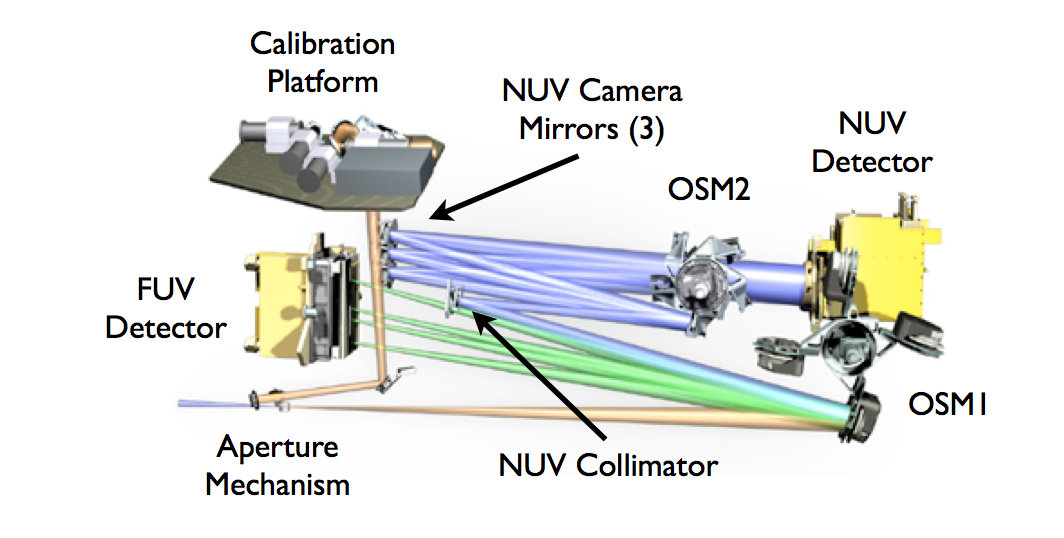
\includegraphics[width=\linewidth]{cos_optical.png}
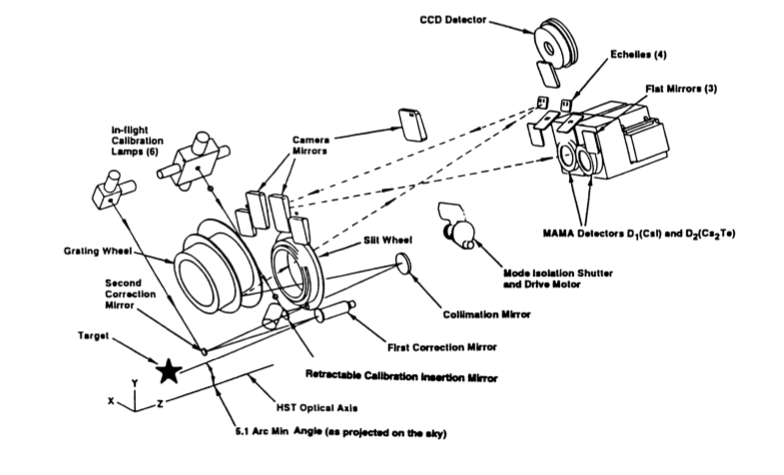
\includegraphics[width=\linewidth]{stis_optical.png}
\caption{Picture are the optical paths and elements of the two spectrographs on HST.  Though built on similar principles, the designs are very different.  \textit{(Top)} COS optical path.
\textit{(Bottom)} STIS optical path.}
\label{fig:x1d_2}
\end{minipage}
\end{figure}

%\begin{figure}[htbp!]
%\begin{center}
%\begin{minipage}[b]{.9\linewidth}
%\begin{center}
%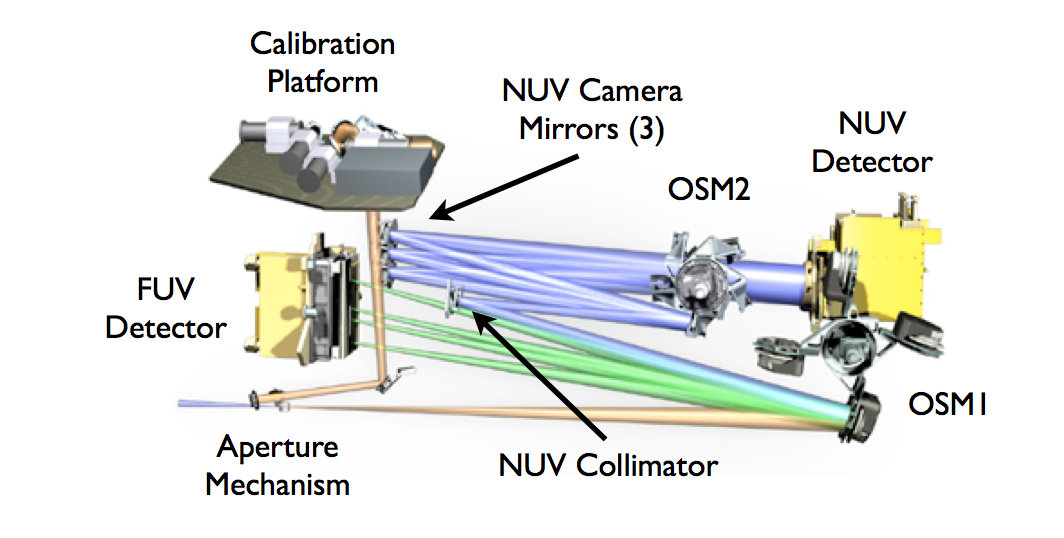
\includegraphics[width=\linewidth]{cos_optical.png}
%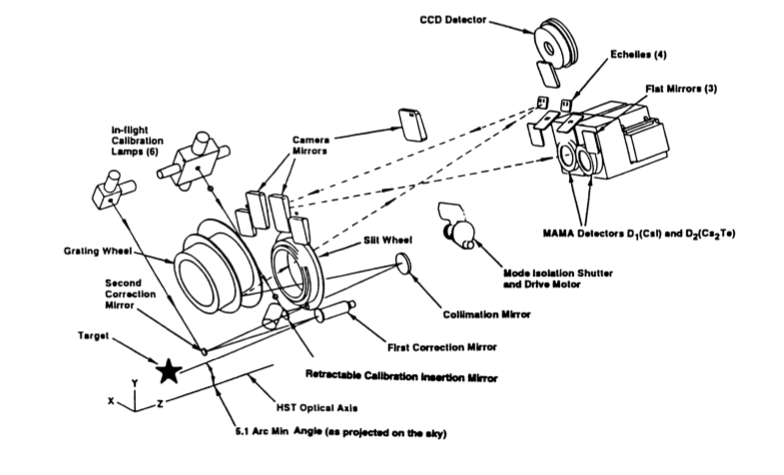
\includegraphics[width=\linewidth]{stis_optical.png}
%\caption{Picture are the optical paths and elements of the two spectrographs on HST.  Though built on similar principles, the designs are very different.  \textit{(Top)} COS optical path.
%\textit{(Bottom)} STIS optical path.}
%\label{fig:x1d_2}
%\end{center}
%\end{minipage}
%\end{center}
%\end{figure}

\section{Uses of Spectroscopy}
Spectroscopy is a very powerful tool used to probe the inner workings of distant objects.  It allows astronomers to measure chemical composition, redshifts, relative velocities, absorption systems, to name a few.

\section{Space-Based Spectroscopy}
\subsection{So many more wavelengths!}
Astronomy from the ground is inhibited by the Earth's atmosphere.   The elements that make up the atmosphere are only transparent to certain wavelength ranges, and so to observe any of the other ranges one must observe from space. See ~\ref{fig:atmo_trans}.

\begin{center}
\begin{figure}[htbp]
\begin{center}
% scale and angle values to be adjusted
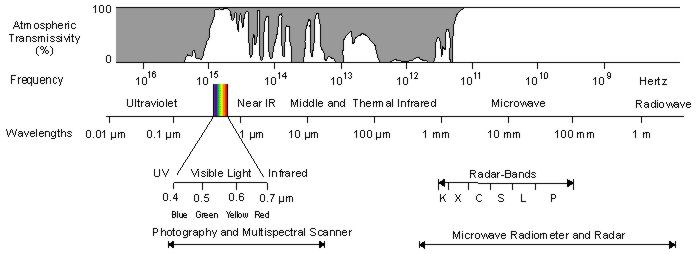
\includegraphics[scale=0.9, angle=0.0]{atmo_trans.jpg}
\caption{Atmospheric transmission with wavelength.  The low transmission at at many wavelengths, particularly UV and shorter, necessitates space based observations.}\label{fig:atmo_trans}
\end{center}
\end{figure}
\end{center}

\subsection{Airglow Lines}
The orbit of HST is close enough to earth to still encounter significant atmospheric effects.  One of the largest of these effects is the presence of emission lines caused by Earth's atmosphere.  The figures below show two of the more prominent lines, Lyman Alpha and Oxygen I.  Both of these features show variability on long and short timescales, with the former changing as HST passes through orbital day and night, and the latter changing as the solar cycle and the earth environment makes large scale changes to atmospheric size, density, etc.  

STIS has the ability to use small slits, and thus to remove much of the contamination from the airglow lines.  COS, however, has a fixed, large, aperture that cannot be used to filter out airglow.  Some filtering can still be done for COS data, but only by removing the part of the exposure that was taken during times of particularly strong airglow emission, such as orbital day. Strong airglow lines have led to the degradation of the COS FUV detector- to combat the damage done, the FUV spectra are periodically shifted up and down in XD (cross-dispersion) to expose on pristine portions of the detector.

\begin{figure}
\begin{minipage}[b]{0.5\linewidth}
\centering
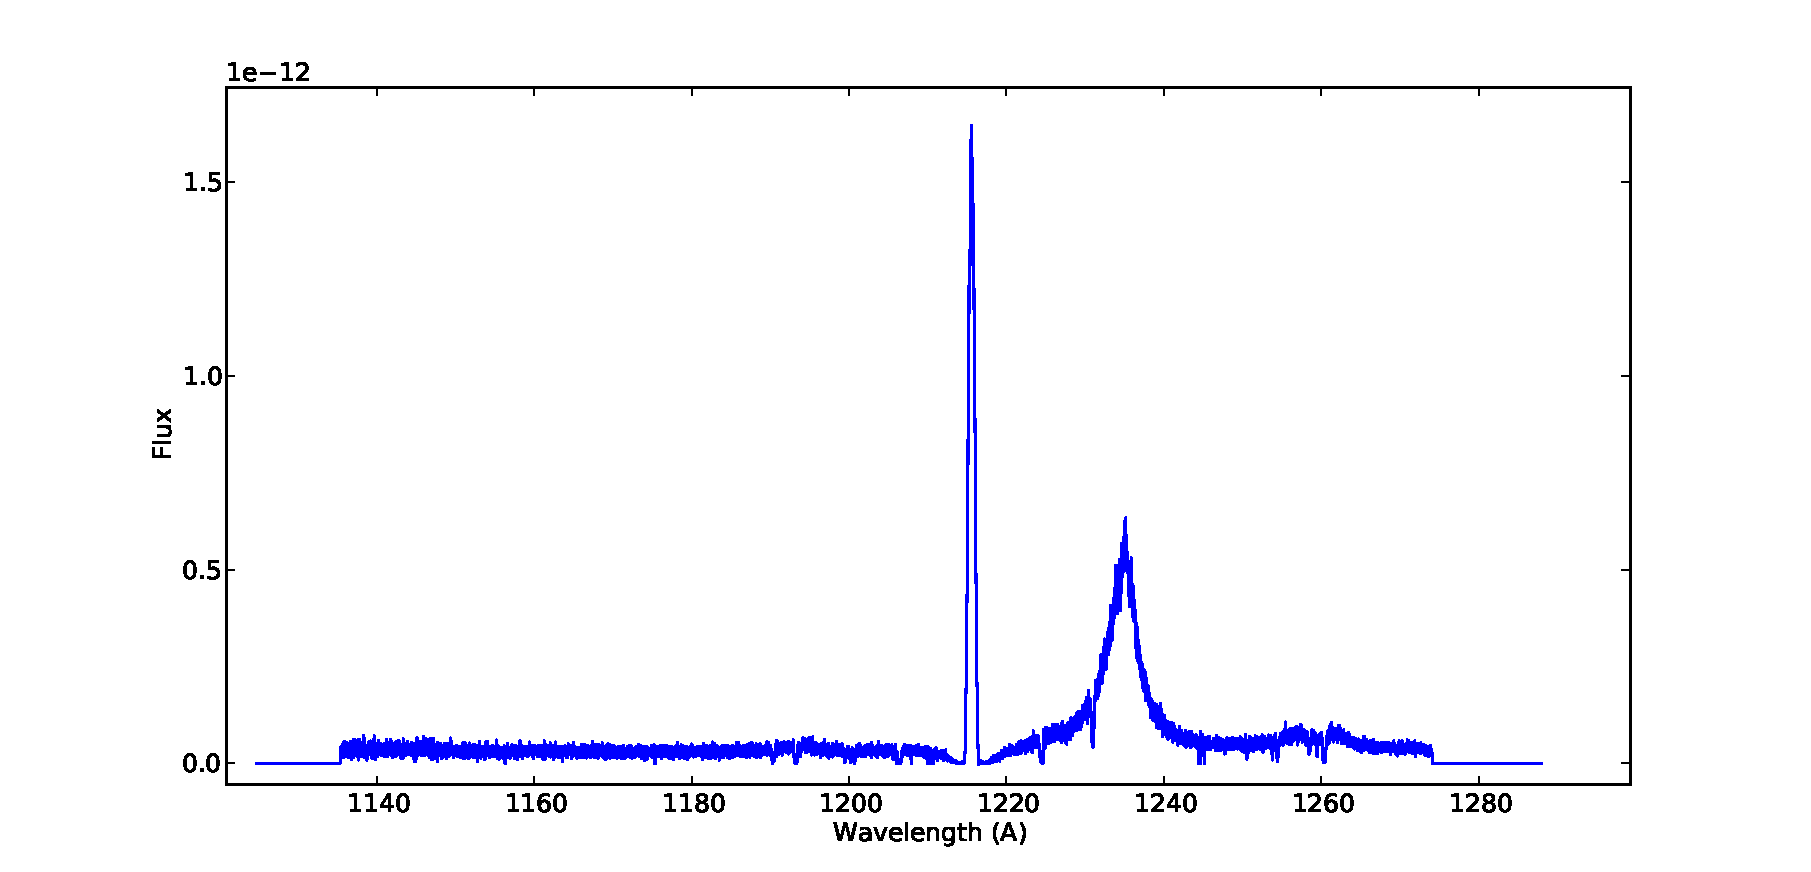
\includegraphics[width=\textwidth]{lya.pdf}
\caption{Geocoronal Lyman Alpha airglow is shown at 1216 \AA.}
\label{fig:geo1}
\end{minipage}
\hspace{0.5cm}
\begin{minipage}[b]{0.5\linewidth}
\centering
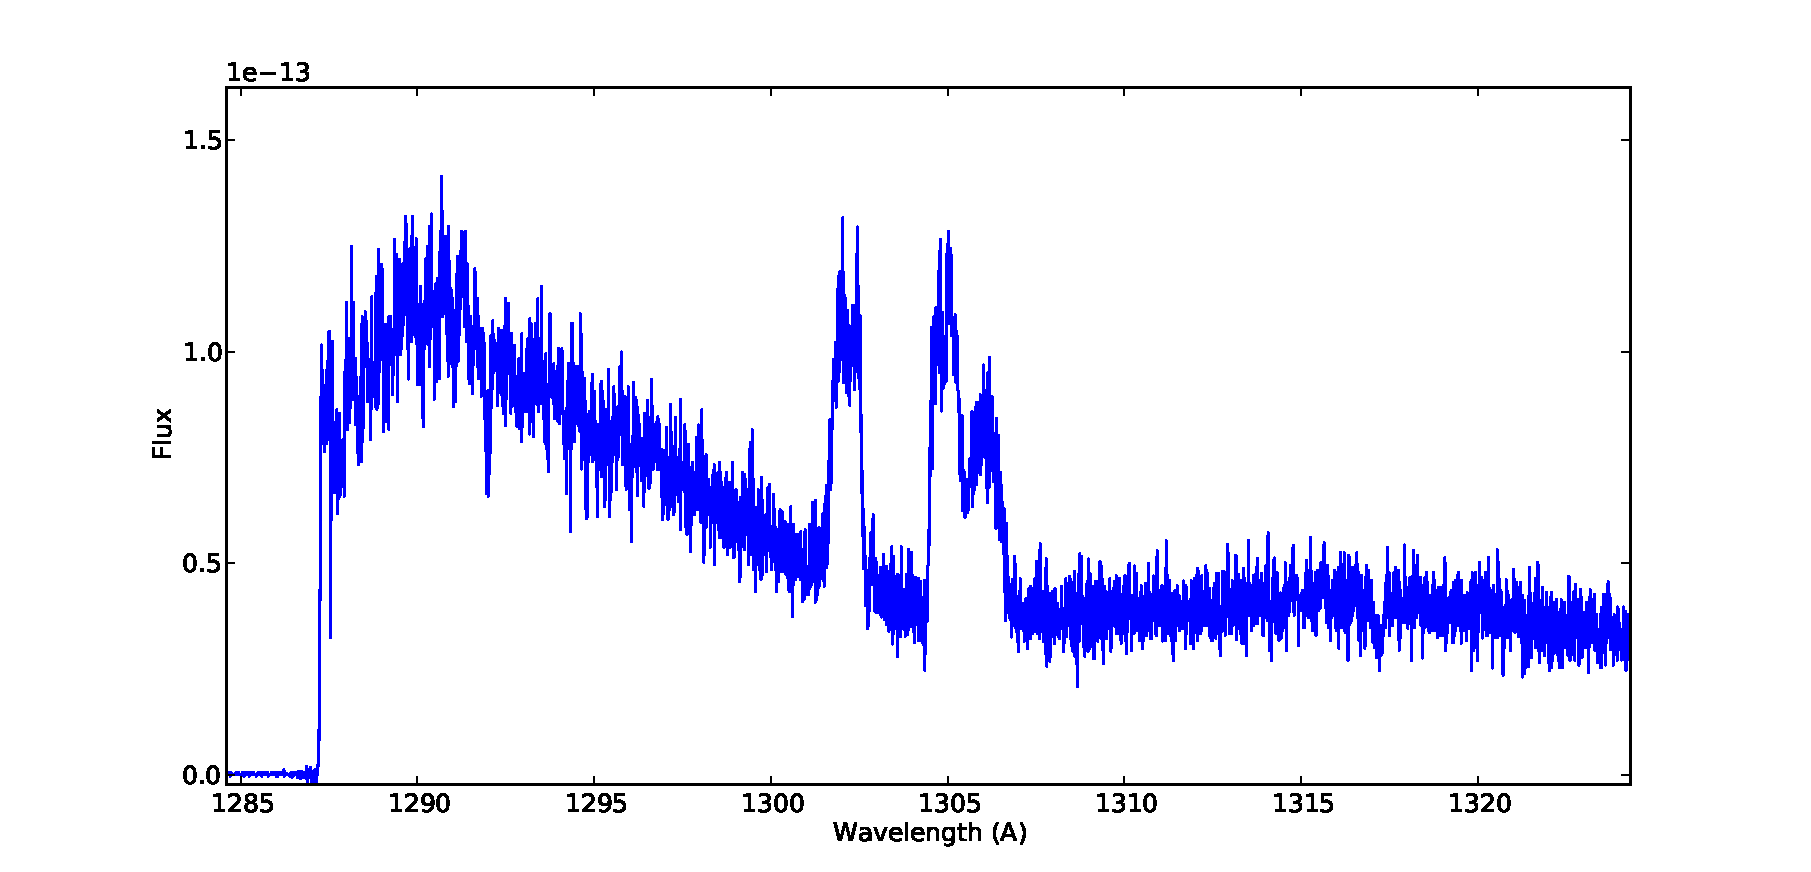
\includegraphics[width=\textwidth]{OIII.pdf}
\caption{Geocoronal Oxygen I airglow between 1300 and 1310 \AA.}
\label{fig:geo2}
\end{minipage}
\end{figure}


\subsection{UV Instrumentation}
Ultraviolet astronomy often requires different detectors than the typical Charged Couple Devices (CCDs).  HST employs two different kinds of UV detectors; Multi-Anode Microchannel Arrays (MAMAs), and an open face Microchannel Plate (MCP) with a Cross Delay Line Anode (XDL).  The MAMA detectors are employed in the FUV and NUV channels of STIS and the NUV channel of COS, \textcolor{red}{while the XDL is only used in the COS FUV channel.} 
%with the XDL only being used in the COS FUV channel.  

These detectors act very differently when compared to CCDs.  The most glaring difference is that these detectors are photon-counting devices.  This means that each incoming photon is uniquely observed by the instrument electronics.  This allows for some great flexibility, and great complexity, in processing of the data.  Data taken in TIME-TAG mode (default on COS, optional on some STIS modes), records the location and time of each photon event.  This means that data can later be screened not just in x,y location, but in time as well.  

UV detectors also experience an incredibly low background rate.  The FUV detector on COS, for example, has a mean dark count rate of $\sim 3.0x10^{-6} cnts/sec/pixel$.   To put this in perspective, in even very long exposures most pixels in the COS FUV detector do not have a single dark count.  

For a far more complete introduction to COS and STIS, along with any other HST instrument, please see that instrument's Instrument Handbook.

\subsection{Differences between COS and STIS}
While both of HST's spectrographs, COS and STIS, overlap in spectral range, there are still many unique advantages to each instrument that will dictate which is the best choice to achieve a program's goals. The FUV throughput, spectral resolution, and wavelength coverage of most COS modes is much higher than that of STIS. In addition, new "blue mode" COS configurations allow observations from the hydrogen Lyman limit (912 \AA) to Ly$\alpha$ (1216 \AA), far surpassing the wavelength range of STIS. The NUV capabilities of both instruments are comparable with the exception that it is easier to obtain broader NUV wavelength coverage with STIS. Generally speaking, STIS is better suited for observing extended sources than COS. Conversely, the COS instrument is optimized to observe point-source objects. The high-dispersion echelle modes of STIS offer resolving powers of up to $R \sim 200,000$. The significantly lower dark rates of COS make it a better choice when observing faint sources. 

Both detectors, however, share a number of features. Both instruments can observe using TIME-TAG mode, recording the time of each photon's arrival. Both COS and STIS MAMA detectors have brightness limits that ensure the safety of the instruments.
\chapter{Working with Spectra: Exercises}
\label{ch:using_data}

\section{HST Spectral Data}
For HST spectral data, there are three types of files; raw, intermediate, and products.  Raw data has undergone no processing besides generic conversion from spacecraft data to FITS, and include \_rawtag, \_rawaccum, and \_rawacq files for COS and \_raw, \_tag, and \_wav files for STIS.  Intermediate products are files produced  by each instrument's calibration pipeline on the way to extracting a spectrum. There are many of these for both COS and STIS, but main ones include \_corrtag files for COS, \_crj and \_sfl for STIS, and \_flt files for both. Products for spectrographs are fully calibrated, extracted spectra and typically end in \_x1d.fits. See the Instrument Data Handbooks for a full list of all data file types. 

{\color{blue} {\sf\small EXERCISES}} \\
Retrieve two datasets,  lbgu17qnq and o8k401010 from the archive. Be sure to retrieve both uncalibrated and calibrated products.  To get lbgu17qnq you will need to search for the association name "lbgu17010" instead of the dataset name, and download all the files it returns (sorry, COS is weird).  One of the calibrated products for both COS and STIS are the \_x1d files. We will examine both \_x1d files using Python (feel free to use your language of choice). You will need to repeat each of these steps for both COS and STIS files.\\

First, look at the primary headers and identify what type of detectors and observation modes each of these exposures used for what targets.
\begin{alltt}
python> from astropy.io import fits 
python> fits.getheader(file_name, 0)
python> detector = fits.getval(file_name, "detector", 0)
python> obsmode = fits.getval(file_name, "obsmode", 0)
python> target = fits.getval(file_name, "targname", 0)
\end{alltt}

To determine if there are differences in the data, you must open the file. Look closely at the file dimensions- the FUV detector of COS is split into two segments, A and B.
\begin{alltt}
python> hdulist = fits.open(file_name)
python> hdulist.info()
\end{alltt}
The science data can be easily analyzed by looking in the extension containing the science information. You can determine the columns in the data extension and their formats and units.
\begin{alltt}
python> data = hdulist[sci_ext].data
python> data.names
python> data.columns
\end{alltt}

{\bf \color{blue} Exercise \arabic{exercise} \stepcounter{exercise}}:  \\
%{\bf What detector was used in the STIS observation? What about the COS observation? What were the observation modes used? What target was observed?\\ 
%What are the names of the columns in each file?\\}
{\bf For each instrument: What detector was used? What observation mode was used? What target was observed? List the names of the columns in each file.}

{\bf \color{blue} Exercise \arabic{exercise} \stepcounter{exercise}}:  \\
%{\bf Open the STIS raw file and both COS rawtag files (there is one for each segment). What is different between the two files? Why are these differences present?\\
%Hint- look again at the OBSMODE header keywords.}
{\bf Open the STIS raw file and both COS rawtag files (there is one for each segment). What is different between the format of the two files? Why are these differences present? (Hint--look again at the OBSMODE header keywords. What does it mean to be taken in TIME-TAG rather than ACCUM?)}

\section{Calibration}
The calibration pipelines for COS and STIS, CalCOS and CalSTIS respectively, are available in python. (They can also be found in the stsdas.hst\_calib package of IRAF/PyRAF, and CalSTIS can be run from the unix shell, if you are so inclined). The calibration pipelines themselves have very limited optional arguments, and very few will effect the data. Most of the ways to change how data is calibrated is accessed by editing header keywords in the raw files. 

All of the calibration files (reference files) used by the calibration pipelines are located on central storage, and the pipelines themselves look to environment variables to find them. If you have not already done so, you will need to set environment variables: oref for STIS, and lref for COS (see the example below). If you haven't already set these in your shell file, it would be benificial to do so now. You will notice, as you begin your work, that STIS datasets always begin with the letter `o', and COS always begin with the letter `l'.  Each instrument has a letter assigned to it, and that is where the reference file directories get their names.
\begin{alltt}
> set oref '/grp/hst/cdbs/oref/'
> set lref '/grp/hst/cdbs/lref/'
\end{alltt}

You have already received calibrated products from the archive, but let's calibrate some data ourselves by using the pipelines.  It is always a good idea to write to screen the trailer file that a pipeline creates- they are step-by-step records of how the data were calibrated and will record any errors that occurred. The steps below are done in python, but you are welcome to calibrate data within IRAF/PyRAF. In IRAF/PyRAF you can get information on the different parameters for both CalSTIS and CalCOS by typing ``help calcos" or ``help calstis". You will need to specify a different output directory to make sure that the pipelines will not overwrite the data you retrieved from MAST.

The pipelines can be imported and run in python as shown:
\begin{alltt}
python> from stistools import calstis
python> calstis.calstis(file_name, verbose = "Yes", outroot="output_dir/")

python> import calcos
python> calcos.calcos(file_name, outdir="output_dir/")
\end{alltt}

Recall looking at the column names before--you can access the data for each of those columns by indexing the science data extension and the column name. Don't forget that COS will contain 2 rows instead of 1 like STIS. If you want to combine both of those pesky COS segments into one array, use ravel(). 
\begin{alltt}
python> your_cos_wavel = data["wavelength"]
python> your_cos_flux = data["flux"]

python> flat_wavel = your_cos_wavel.ravel()
python> flat_flux = your_cos_flux.ravel()
\end{alltt}
Now, let's plot some data. If you are plotting STIS data, you will need to plot wavel[0] and flux[0]. If you did not flatten your COS data, you will need to plot each segment by calling wavel[0]/flux[0] for the B segment and wavel[1]/flux[1] for the A segment. If you did flatten your COS data, simply plot wavel and flux. Let's add some labels and a title to spruce up our plots too.
\begin{alltt}
python> from matplotlib import pyplot
python> pyplot.plot(wavel, flux)
python> pyplot.xlabel("Wavelength [$\textbackslash AA$]")
python> pyplot.ylabel("Flux")
python> pyplot.title("COS MARK1044")
\end{alltt}
Isn't that a nice looking plot!

{\bf \color{blue} Exercise \arabic{exercise} \stepcounter{exercise}}:  \\
{\bf Using the STIS and COS raw files as input, calibrate the data yourself by using CalSTIS and CalCOS respectively. Examine the wavelength and flux levels in the products you produced compared to the products you retrieved from the archive. Are they identical? On separate plots, plot the STIS and COS spectra from the x1d files.}

{\bf \color{blue} Exercise \arabic{exercise} \stepcounter{exercise}}:  \\
{ \bf Say you have decided that the standard pipeline is not doing a good job of background subtracting the data.  Turn off the BACKCORR calibration switch in the primary (0th) extension header of the COS and STIS raw files and recalibrate.  You can change the switch by changing the BACKCORR keyword value from "PERFORM" to "OMIT" (Hint: There are many ways to do this, but if using python try using fits.setval). Produce a plot comparing the COS spectra with BACKCORR turned on and with it turned off. Produce the same plot for the STIS data. What, if anything, has changed?} 
\section{Smoothing/Convolving}
The COS data you have is at a much higher resolution than that of STIS.  We would like to directly compare the two datasets, so it would be great if they were on more even footing.  

{\bf \color{blue} Exercise \arabic{exercise} \stepcounter{exercise}}:  \\
{\bf Smooth the COS data with a boxcar filter using your favorite convolution function.  Try different box sizes and see what size approximately matches the two spectra the best.  (Just approximate is fine, this is just for an introduction). It is best not to use a box size greater than 15, or signal is smoothed out along with noise. Below is one way to do this in python. Produce a plot of the smoothed COS spectrum.}
\begin{alltt}
python> from stsci.convolve import boxcar
python> smooth_flux = boxcar(flux, (boxcar_size,) )
\end{alltt}

%{\it OPTIONAL Exercise \arabic{exercise} \stepcounter{exercise}:  \\
%If you feel up to it, use the LUCY deconvolution task in iraf/Pyraf to deconvolve the LSF from the COS data and compare with that of STIS.} \\


\section{Signal to Noise}
The signal to noise ratio (S/N) of a dataset is an important statistic to be able to estimate.  If the S/N is too low to detect your feature of interest, then attempting to use your dataset is a waste of your time. The signal can be approximated with a low order polynomial fit to a continuum region where there are no absorption or emission lines, and the noise can be approximated as the standard deviation of the data - fit.  Some useful functions in Python are numpy.polyfit, numpy.poly1d, and numpy.std. 

{\bf \color{blue} Exercise \arabic{exercise} \stepcounter{exercise}}:  \\
{\bf Determine the signal to noise of the continuum of both the COS and STIS spectra. Which dataset has the better signal to noise, COS or STIS? Does this number make sense with what your eye is seeing?} 

\section{Interpolation}
Directly comparing two spectra in wavelength space cannot be done, apart from visually, unless both datasets have the same wavelength scale.  Interpolating one spectrum onto another wavelength scale will allow you to do far more useful calculations such as dividing, subtracting, etc. Below is the syntax for using one linear interpolation algorithm from numpy, which gives you interpolated fluxes on the wavelength scale of wavel1.
\begin{alltt}
python> import numpy as np
python> flux2_interpolated = np.interp(wavel1, wavel2, flux2)
\end{alltt}

{\bf \color{blue} Exercise \arabic{exercise} \stepcounter{exercise}}:  \\
{\bf Perform a linear interpolation of the STIS dataset onto the wavelength scale of the COS dataset.  Then divide the two spectra by each other to see where the two differ. Produce a plot of the divided spectrum.} 
%\section{Fitting Features}
%Identifying and fitting features in spectra is the backbone of practical spectroscopy, and leads to the determination of much more than simply if an element is present or not.

%There are many fitting tasks available in a variety of languages.  A very powerful one in IRAF is the SPLOT task.  See the manual for more information.

%\subsection{Redshifts}
%In measuring redshifts, line centroids are more important than anything else, so high-resolution spectroscopy is very important, and blended lines should not be used if any alternatives are available. Doublets are especially useful in this case because the ratio of the wavelengths does not vary with redshift.

%{\color{blue} {\sf\small EXERCISES}} \\
%{\it Exercise \arabic{exercise} \stepcounter{exercise}:  \\
%Find the redshift of the Quasar in one of your datasets by comparing the rest wavelength of Lyman alpha to its emitted wavelength.  NOTE: The emitted lyman alpha line is the broad feature to the red side of the geocoronal 1216 \AA line.  } \\

%\subsection{Relative Velocities}
%As with redshift above, but generally requires much higher precision, and looks for time vari- ability. And yes, it�s much more complicated than my discussion here implies, but this is a general introduction.

%\subsection{Chemical Abundances}
%Here, equivalent width is the most important thing, as are taking measurements of multiple lines with different oscillator strengths. In the case of absorption lines along long sightlines, be careful to avoid problems caused by line blending (which will distort the equivalent width measurements.).

%\subsection{Detecting Absorption Systems}
%By definition, absorption systems (e.g. non-luminous interstellar gas clouds) are difficult to examine via imaging. However, when such systems are found in front of bright background sources (stars, galaxies, or quasars), they can be used to examine the interstellar medium (ISM) in ways that are difficult to accomplish otherwise. In these cases, high-resolution spectroscopy is important (if available) to resolve multiple components, and in order to deal with blended lines. UV spectroscopy allows the H I column density to be determined, which provides information about which metal lines will be dominant. Relative abundances of metals at various ionization states can be used to model the background radiation level.

\chapter{Assignments}
\label{ch:assignments}

{\bf NOTE: Please do not perform the following assignments unless you are assigned to.}

\section{Spectroscopy of RECX-1}

RECX-1 is a T-Tauri star that was observed as part of Program 11616. During these observations, the star experienced a flare. Your assignment here involves taking these COS observations, determining when the flare occurred, and determining which parts of the star's spectrum were affected by the flare

Tools that may be useful for this include using \texttt{splittag} to separate the corrtag data by time or spatial location, in order to look for count rate changes. In addition, the \texttt{x1dcorr} task allows split datasets to be extracted. {\color{red}{These are located in the \texttt{costools} package in python and pyraf. There is additional documention located online, but the basics of calling these tasks in python are as follows: \\

\texttt{python> from costools import splittag \\
python> splittag.splittag("rootname\_corrtag\_a.fits", "output\_filename", time\_list = "0, 250, 500, 750, 1000")} \\
or equivalently: \\
\texttt{python> splittag.splittag("rootname\_corrtag\_a.fits", output\_filename", starttime = 0., increment = 250., endtime = 1000."} \\

To finish the pipeline extraction, run the x1dcorr task: \\

\texttt{python> from costools import x1dcorr\\
python> import glob\\
python> for corrtag\_file in glob.glob("*output\_filename\_corrtag*"): \\
python> ... x1dcorr.x1dcorr(corrtag\_file)} }}

\begin{enumerate}
	\item Retrieve Program 11616 Visit 32.
	\item Determine approximately when the flare started (assuming that it started after the observations began),
		and when the flare ended (assuming that it ended whilst the observations were still ongoing). \textbf{NOTE} that any
		Lyman-$\alpha$ or O~{\sc i} emission is geocoronal emission from the Earth's atmosphere and not intrinsic to RECX-1. 
		Note also that the effects of the flare are visible in the star's emission lines rather than its continuum. {\color{red}{\textbf{Additional help--}once you have split the data by an appropriate time interval to see the flare, overplotting wavelength vs. flux in the multiple x1d files might help to see any differences in the spectrum over time.}}
	\item A number of emission lines can be seen in the star's spectrum. Which elements and ionization states do these
		lines correspond to?
         \item {\color{red}{What are some common elements that produce emission lines that are seen in T-Tauri stars in the UV? At what wavelengths, if at all, do you see these in
                  RECX-1?}}
	\item Are all of the lines affected in the same way by the flare?
\end{enumerate}

\section{Chemical Abundances in AO~0235$+$164}

\begin{enumerate}
	\item Retrieve Program 7294 Visits 01 and 02. (bonus: if you're up to dealing with FOS, retrieve visit 01 of 
		Program 6217 as well). In this case, retrieving the processed data should be sufficient.
	\item There is a damped Lyman-$\alpha$ system (DLA) in this sightline. What is its redshift? What is the 
		N(H~{\sc i})?
		\begin{center}

     		\begin{figure}[htbp]
		\begin{center}
		% scale and angle values to be adjusted
		%\includegraphics[scale=0.7, angle=0.0]{dla.pdf}
		%\caption{The Damped Lyman Alpha system is seen around 1850 \AA. }\label{fig:atmo_trans}
                  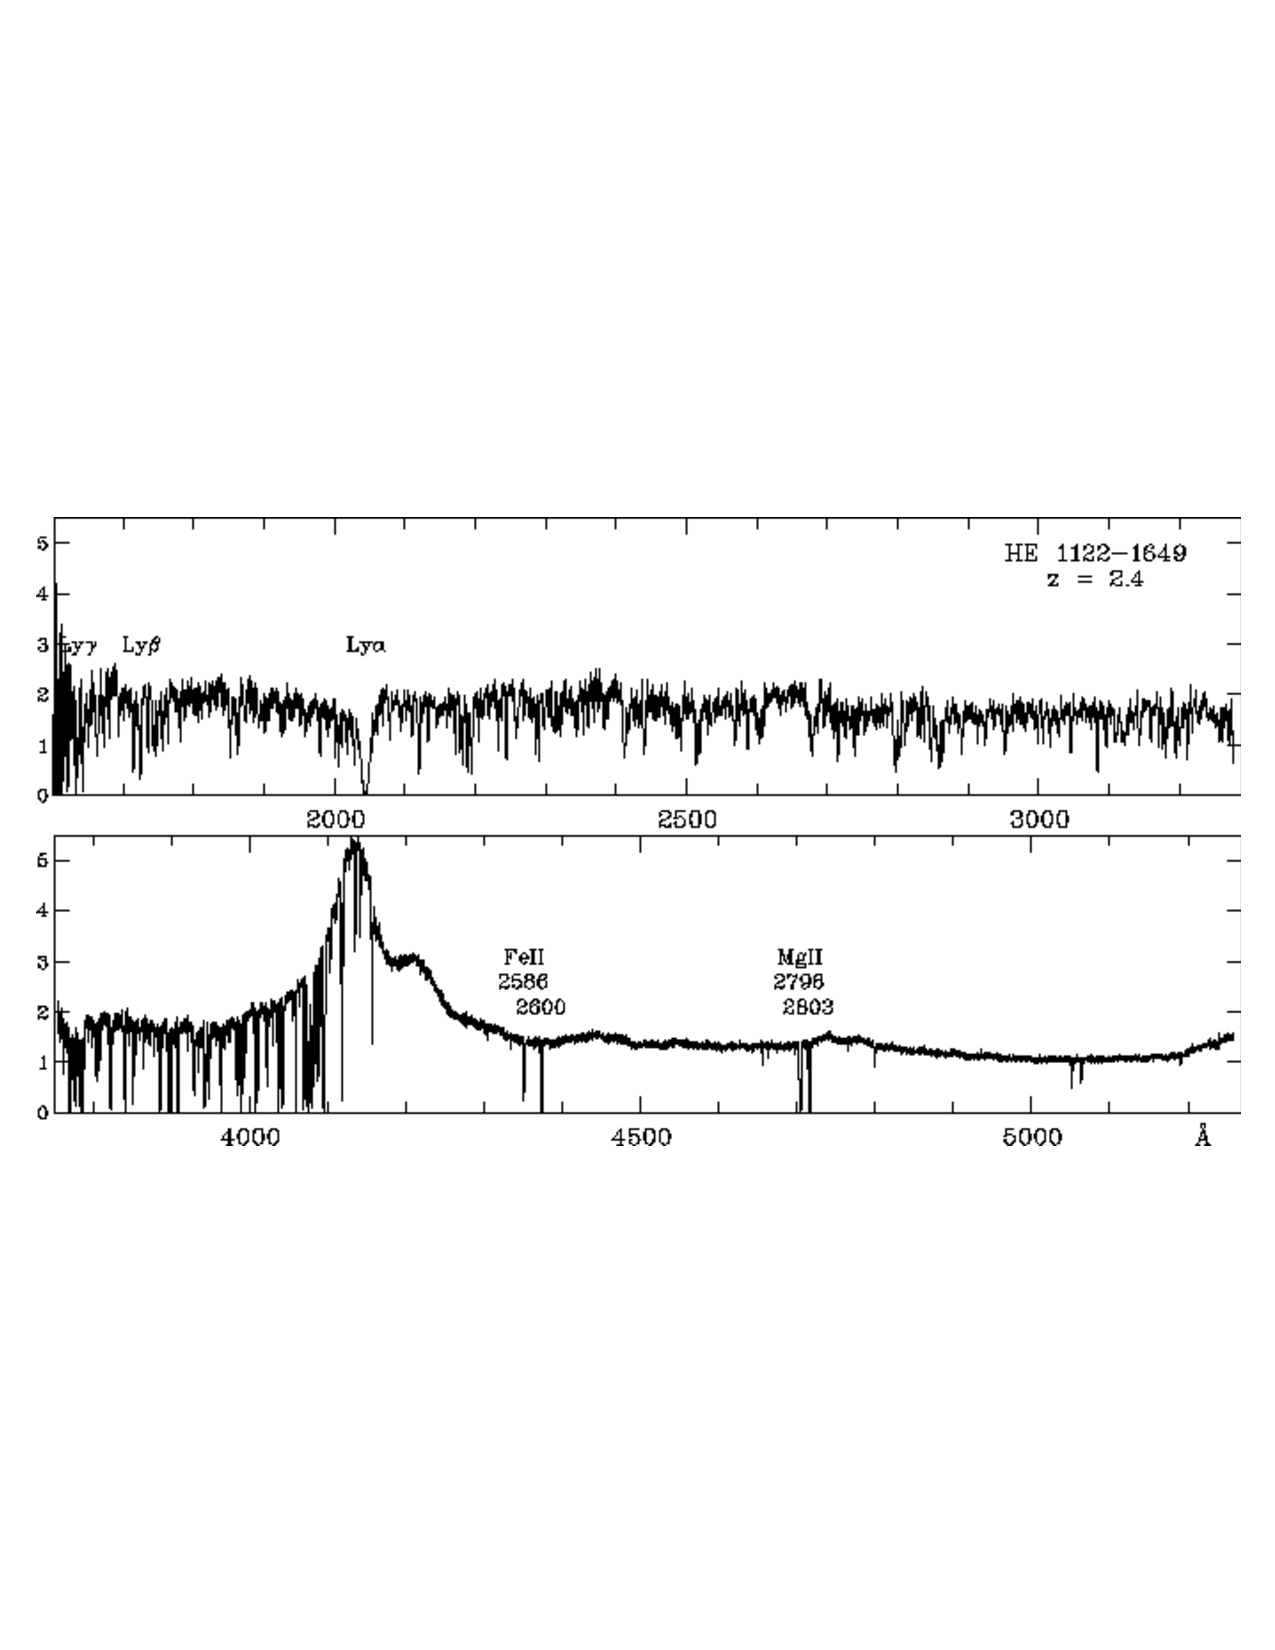
\includegraphics[scale = 0.7, angle=0.0]{ex2_spectrum.pdf}
                  \caption[Fake Caption?]{{\color{red}{An exmaple spectrum of a different QSO UV spectrum with a different redshift. The Lyman Alpha and Magnesium II lines are labeled, which should help you find these lines in AO 0235+164's spectrum \footnotemark.}}}
		\end{center}
		\end{figure}
		\end{center}
         \footnotetext{{\color{red}{{\it{Absorption line spectra of the UV bright z=2.4 QSO HE 1122-1649}}\\
         S. Köhler, A. de la Varga and D. Reimers\\
         Hamburger Sternwarte, Gojenbergsweg 112, 21029 Hamburg, Germany}}}

	\item What is the Mg~{\sc ii} column density associated with the DLA? {\color{red}{Use equation 4.26 as well as the \texttt{splot} task in pyraf.}} Are the Mg~{\sc ii} lines likely 
		saturated {\color{red}{based off what a saturated line looks like in Figure 4.1?}} What redshift do you derive from the Mg~{\sc ii} doublet? Is it significantly different from
		the redshift derived from H~{\sc i}? Which would you trust more, and why?
	%\item Can you detect Mg~{\sc i} lines? What column density do you derive for Mg~{\sc i}? How accurate do you
	%	think it would be to assume that all of the magnesium in the system is singly ionized?
	\item Zn~{\sc ii} and Cr~{\sc ii} are often used to derive metallicities and dust abundances for DLAs. Can
		you detect lines belonging to either? {\color{red}{Hint: Zn~{\sc ii} has rest wavelengths at 2026\AA and 2062\AA(blended) and Cr~{\sc ii} has rest wavelengths at 2056\AA and 2066\AA. Calculate where the observed lines should fall using the redshift in question 1 or 2 of this exercise.}}
	%\item What other metal lines can you detect with a high degree of confidence? How metal-rich is this DLA based
	%	on these atoms?
         \item {\color{red}{Are there any other metal lines you can detect with a high degree of confidence? By calculating the rest wavelengths and using the NIST spectral database or somewhere you can find element emission rest wavelengths and relative intensities, see what these lines likely correspond to. Remember that any airglow lines aren't intrensic to the target and therefore won't be redshifted.}} How metal-rich would you say this DLA is based on these atoms?
\end{enumerate}
\chapter{Physical Basis of Spectroscopy}
\label{ch:theory}

Astronomical spectroscopy can be seen as the study of emission and absorption lines against a background continuum. The material provided here omits much of the necessary physics background, but provides at least a basic introduction to spectroscopy.

\section{Spectral Lines}

\subsection{Transition Probabilities}

The Einstein coefficients are defined as the probabilities for spontaneous transitions (A for emission, and B for absorption). The inverse of these coefficients give the radiative lifetimes (e.g. 1/A is the time for a transition to spontaneously decay).
\begin{equation}
	A_{ji} = \frac{8 \pi h B_{ij} g_i}{g_j \lambda^3} \\
\end{equation}
\begin{equation}
	B_{ij} = \frac{f_{ij} e^2 \lambda}{4 \epsilon h c m_e}
\end{equation}
where $f$ is the oscillator strength, and $g$ the statistical weight of states $i$ and $j$ respectively. These equations treat the transition as if it were a bound harmonic oscillator, and asks how efficient the transition is at absorbing energy. Often, the $g$ and $f$ values are tabulated together:
\begin{equation}
	g_i f_{ij} = A_{ji} g_j \lambda^2 \left(\frac{4 \epsilon c m_e}{8 \pi e^2}\right)
\end{equation}
The oscillator strength is a transition probability which can be experimentally or theoretically derived from Quantum Mechanics. Typical A values are $10^8$--$10^9$~s$^{-1}$ for permitted resonance transitions, $\sim 10^3$~s$^{-1}$ for semi-forbidden lines, and $\sim 10^{-3}$~s$^{-1}$ for forbidden lines. Thus, forbidden lines are usually seen only in diffuse environments where the time between collisions is longer than about 1000 seconds.

\subsection{Local Thermodynamic Equilibrium}

The distribution of atomic states and energies for LTE is given by statistical mechanics. The Boltzmann equilibrium provides the relative number of atoms in an excited state, $j$, compared with the ground state ($j=1$) at a given temperature, $T$:
\begin{equation}
	\frac{N_j}{N_1} = \frac{g_j}{g_1} \exp\left(\frac{-\Delta E}{kT}\right)
\end{equation}
where $\Delta E$ is the energy difference between the ground and excited states, and $k$ is the Boltzmann constant ($k = 1.38 \times 10^{-16}$~erg~K$^{-1}$). The energies for hydrogen may be approximated by the empirical formula
\begin{equation}
	E_n = \frac{-h c R_H}{n^2} = -13.6{\textrm eV}\frac{1}{n^2}
\end{equation}

The energies of atoms will follow a Maxwell-Boltzmann distribution, which can be expressed as a function of either temperature or velocities:
\begin{equation}
	n(E) = \frac{2 N}{\pi^{1/2} (kT)^{3/2}} E^{1/2} \exp\left(\frac{-E}{kT} dE\right)
\end{equation}
which has a most probably energy $kT$, or a most probable velocity $v = \sqrt{(2kT/m)}$. However, LTE is not usually applicable to the interstellar medium (ISM), as low densities mean that a Boltzmann equilibrium is rarely achieved because collisions are too rare. In the ISM, therefore, radiative processes become important. The Maxwellian distribution is usually applicable to the ISM.

\section{Measuring Absorption and Emission Lines}

Lines are often measured via their equivalent width, $W$, using the relationship:
\begin{equation}
	W = \int{\frac{I_0 - I_{\lambda} d\lambda}{I_0}}
\end{equation}
where $I_0$ is the continuum intensity and $I_{lambda}$ the intensity at the wavelength $\lambda$. Note that, using this definition, emission lines will have negative $W$ whilst absorption lines will have positive $W$. Equivalent width can most easily be thought of as the area which would be taken up by the line on a normalized spectrum ($I_0 = 1$). In the case of observed spectra there will be noise, which will in turn lead to a detection limit. The n$\sigma$ detection limit is
\begin{equation}
	W_{\rm lim} = \frac{n \times d \times \sqrt{M}}{\rm SNR}
\end{equation}
where $d$ is the dispersion (pixel width in \AA), and $M$ the number of pixels across the line. In the case of unresolved lines, this can be approximated to
\begin{equation}
	W_{\rm lim} = \frac{n \times {\rm FWHM}}{\rm SNR}
\end{equation}

The width of a line is usually expressed in km/s as either the velocity dispersion ($\sigma$) or the FWHM. In the case of a Gaussian distribution the two quantities are related, with ${\rm FWHM} = 2\sqrt{2\ln2}\sigma = 2.355\sigma$. Widths are often expressed in terms of the Doppler width, $b$, caused by thermal and turbulent broadening, where:
\begin{equation}
	b = \sqrt{2}\sigma = \frac{\rm FWHM}{2\sqrt{\ln2}}
\end{equation}
For emission lines, the flux is often quoted instead of the equivalent width, either in units of $F_{\nu}$ (ergs s$^{-1}$ cm$^{-2}$ Hz$^{-1}$ (Jy)), or $F_{\lambda}$ (ergs s$^{-1}$ cm$^{-2}$ \AA$^{-1}$) where $F_{\lambda} = F_{\nu} c/\lambda^2$. Graphs may be plotted with $\lambda F_{\lambda}$, or total energy.

\section{The Voigt Profile}

Spectral lines are broadened by various processes, including pressure broadening (more important in stars), thermal and turbulent broadening, and natural broadening (which occurs due to Heisenberg's uncertainty principle $\Delta E \Delta t \geq \hbar$). Because any transition has a finite lifetime $\Delta t = 1/A_{ji}$, the natural width in terms of frequency is $\Delta \nu_{N} = A_{ji}/2\pi$. Often this natural frequency width is replaced by the damping constant $\Gamma = 2 \pi \Delta \nu_{N}$, which is connected to the radiative transfer probability: for a transition from the ground state, $\Gamma$ is the sum over the Einstein coefficients for spontaneous emission for levels up to the level in question. The absorption cross-section (measure of probability) for natural broadening can then be expressed as:
\begin{equation}
	\sigma_L(\nu) = \left(\frac{\pi e^2}{m_e c}\right)f\frac{\Gamma/4 \pi^2}{(\nu - \nu_0)^2 + (\Gamma/4\pi)^2}
\end{equation}
(ignoring the term for stimulated emission).

Thermal and turbulent motions are combined into the Doppler width, which is assumed to follow a Gaussian distribution.
\begin{equation}
	P(v) = \frac{1}{b \sqrt{\pi}}e^{-(v/b)^2}
\end{equation}
\begin{equation}
	b = \sqrt{b^2_{\rm thermal} + b^2_{\rm turbulent}} = \sqrt{\frac{2kT}{m} + b^2_{\rm turbulent}}
\end{equation}
If $b$ is dominated by thermal broadening, then this simplifies to $b = 12.8 {\rm km/s} \sqrt{T/m}$

Combining Equations 11 and 12 gives an absorption cross-section
\begin{equation}
	\sigma(\nu) = \left(\frac{\pi e^2}{m_e c}\right)f\frac{\Gamma}{4\pi^2}\int^{+\infty}_{-\infty}\frac{e^{-(v/b)^2}dv}{(\nu - \nu_0(1+v/c))^2 + (\Gamma/4\pi)^2}
\end{equation}
This expression can (fortunately) be simplified using the Voigt function, $H(a,u)$
\begin{equation}
	H(a,u) = \frac{a}{\pi}\int^{+\infty}_{-\infty}\frac{e^{-y^2}dy}{(u-y)^2 + a^2}
\end{equation}
where
\begin{equation}
	\Delta \nu = \frac{b\nu_0}{c}; a = \frac{\Gamma}{4\pi \Delta\nu}; u = \frac{c(\nu-\nu_0)}{\nu_0 b}; y=\frac{v}{b}
\end{equation}
Substituting this into Equation 14 gives
\begin{equation}
	\sigma(\nu) = \frac{\sqrt{\pi} e^2 f}{m_e c}\frac{H(a,u)}{\Delta \nu}
\end{equation}
We can now write the line optical depth ($\tau = N \sigma = \ln(I_0/I)$) as
\begin{equation}
	\tau(\nu) = \frac{\sqrt{\pi}e^2}{m_e}\frac{N f}{b\nu}H(a,u)
\end{equation}
or, written as a function of wavelength,
\begin{equation}
	\tau(\lambda) = \frac{\sqrt{\pi}e^2}{m_e c}\frac{N f \lambda}{b}H(a,u) = 1.497 \times 10^{-15}\frac{N ({\rm cm^{-2}}) f \lambda (\text{\AA})}{b ({\rm km~s^{-1}})}
\end{equation}
At this point, it is worth noting that optical depth, unlike intensity, has the advantage that $\tau_{\rm total} = \tau_1 + \tau_2$.

\section{The Curve of Growth}

Having covered all of that (and in rather abbreviated form), we move on to the most important question -- what is the effect of having light incident upon absorbing atoms? The optical depth, $\tau$, described above, is more formally defined as
\begin{equation}
	I(\nu) = I_0(\nu)e^{-\tau}
\end{equation}
\begin{equation}
	\tau(\nu) = N\sigma(\nu)
\end{equation}
where $N$ is the gas column density (cm$^{-2}$). Because $W$ is \emph{defined} as the normalized net flux removed from the beam,
\begin{equation}
	I_0 W = I_0 \int d\nu - \int I(\nu) d\nu
\end{equation}
\begin{equation}
	W = \int(i - \exp[-N \sigma(\nu)])d\nu
\end{equation}
When the optical depth of the cloud is small, $\tau(\nu) = N\sigma(\nu) \ll 1$, so
\begin{equation}
	W = N\int \sigma(\nu)d\nu
\end{equation}
\begin{equation}
	W(\nu) = \frac{\pi e^2}{m_e \nu}N f
\end{equation}
\begin{equation}
	W(\lambda) = \frac{\pi e^2 \lambda_0}{m_e c^2}N \lambda_0 f
\end{equation}
and the equivalent width is directly proportional to the number of atoms along the line of sight. This is the linear portion of the curve of growth, and Equation 26 may be simplified to
\begin{equation}
	N = 1.13 \times 10^{20} \frac{W(\lambda)}{\lambda_0^2 f}
\end{equation}
for wavelengths in \AA.

As the column density increases, the absorption line will eventually become saturated (see Figure~\ref{fig:linetypes}). In the saturated regime, the equation becomes instead
\begin{equation}
	W(\lambda) \sim \frac{2b\lambda_0}{c}\sqrt{\ln\left(\frac{\pi^{0.5}e^2N\lambda_0f}{m_ecb}\right)}
\end{equation}
At this point $W(\lambda) \propto \sqrt{\ln N}$, the flat (or saturated) part of the curve of growth. As can be seen from Figure~\ref{fig:cog}, the precise shape of this part of the curve of growth depends significantly on the $b$-value, causing a degeneracy between $N$ and $W$, and making Voigt profile fitting very uncertain.

Finally, when the column density is high enough ($N \gtrsim 10^{19}$~cm$^{-2}$), the Lorentzian profile of the natural broadening begins to dominate the wings of the absorption line (again, see Figure~\ref{fig:linetypes}). In this ``damped'' regime, $W(\lambda) \propto \sqrt{N}$, and is again independent of $b$-value:
\begin{equation}
	W(\lambda) \sim \frac{\lambda_0^{1.5}}{c}\sqrt{\frac{e^2}{m_ec}N\lambda_0f\gamma}
\end{equation}
Since the only element usually present in large enough quantities to produce damped lines is neutral hydrogen (H~{\sc i}), the column density of neutral hydrogen in a damped environment may be derived as
\begin{equation}
	N = 1.88 \times 10^{18} W^2
\end{equation}
at the rest wavelength.

\begin{center}
\begin{figure}[htbp]
\begin{center}
% scale and angle values to be adjusted
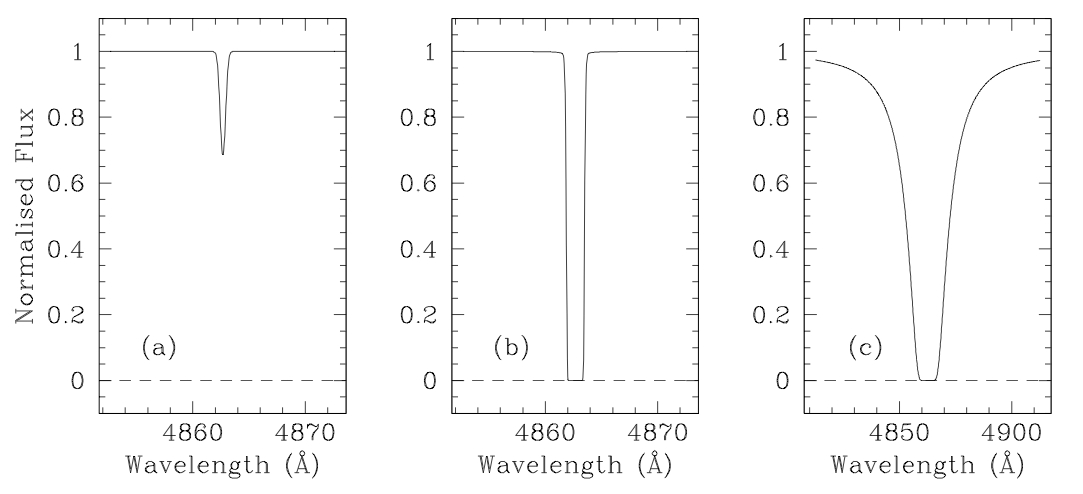
\includegraphics[scale=0.35, angle=0.0]{fig_linetypes.jpg}
\caption{\textsl{Examples of linear (a), saturated (b), and damped (c) absorption lines. All of these lines are Ly$\alpha$ lines redshifted to $z_{abs}=3.0$, with $b = 20$~km/s. $\log N(H~\text{{\sc i}}) = 13 ({\rm a}), 16 ({\rm b}), 20 ({\rm c})$}}\label{fig:linetypes}
\end{center}
\end{figure}
\end{center}

\begin{center}
\begin{figure}[htbp]
\begin{center}
% scale and angle values to be adjusted
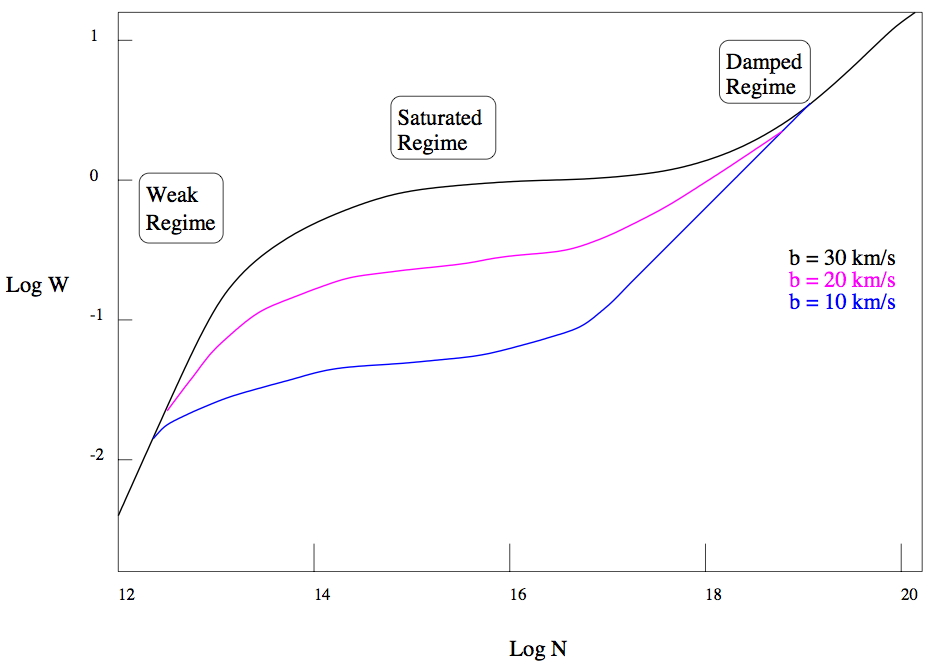
\includegraphics[scale=0.28, angle=0.0]{fig_cog.jpg}
\caption{\textsl{Schematic figure illustrating the curve of growth for Ly$\alpha$ absorption lines for three different $b$-values (Doppler widths).}}\label{fig:cog}
\end{center}
\end{figure}
\end{center}

\section{Redshift}

{\color{red}{Another very important concept in spectroscopy, and astronomy in general, is finding how far away an object is. This can be done by calculating the object's redshift. In order to do this properly, one must know the wavelength at which an element emits/absorbs here at Earth (the rest wavelength) and the wavelength the object in space is emiting that same element (the observed wavelength). From there it is a simple calculation:
\begin{equation}
    z = \frac{\lambda_{obs} - \lambda_r}{\lambda_r} = 1 - \frac{\lambda_{obs}}{\lambda_r}
\end{equation} 

where $\lambda_{obs}$ is the observed wavelength from the object and $\lambda_r$ is the rest wavelength. At non-relativistic speeds this can be approximated to:
\begin{equation}
    z \approx \frac{v_r}{c}
\end{equation}

which gives you an idea of how fast an object is moving away from you.

For objects such as galaxies, sometimes it is possible to calculate the rotation curve as well by using these simple equations. Instead of using the rest wavelength here at Earth, define the center of the galaxy--the bulge is usually the brightest part--to be the rest frame and the opposite edges of the galaxies to be the observed wavelengths. This is just one of many fun examples of ways spectroscopy helps do amazing science.
}}


Redshift increases both $W$ and FWHM by a factor of $(1 + z)$, which may sometimes result in an otherwise unresolved line being resolved (and which will also mean that, even for constant SNR, the detection limit on a line will depend on that line's redshift).

\section{Relative Solar Abundances}

Elemental abundances are often expressed in solar-relative terms, denoted by surrounding the element with square brackets, as shown below:
\begin{equation}
	[Z] = log(N(Z)/N(H)) - log(N(Z)/N(H))_\odot
\end{equation}
Thus, [Zn] = -1.0 would mean that the Zinc is 1/10 as abundant \emph{when compared to hydrogen} in the system of interest as compared to the solar system. In many astronomical systems, it is assumed that N(H)$\sim$N(H~{\sc i}), and that the abundance of the dominant ionization state of the element involved (e.g. Zn~{\sc ii} for zinc) is essentially equal to the abundance of that element as a whole.

Note that solar system abundances may be measured either in the solar atmosphere or in meteoroids, and that these values do not always agree exactly. Note also that, when a pure logarithmic abundance relative to hydrogen is expressed, it may have 13 added to it (by convention, when quoting solar abundances log(X/H) = log(X/H) + 13.00). This won't matter when computing the solar-relative abundance, but is worth knowing so as to avoid confusion.

Relative abundances are also used to compare different metals. For example, [Cr/Zn] is used as a measure of dust abundance because Cr depletes onto dust grains whereas Zn generally does not.


\chapter{Resources}
\label{ch:links}
 
\section{Useful Links }
Below is a list of links to be used as a reference.
\begin{itemize}
\item \url{http://docs.python.org/}
\item \url{http://legacy.python.org/dev/peps/pep-0008/}
\item \url{http://wiki.python.org/moin/HowTo/Sorting}
\item \url{http://ipython.scipy.org/moin/Documentation}
\item \url{http://matplotlib.sourceforge.net/}
\item \url{http://www.scipy.org/Numpy\_Example\_List\_With\_Doc}
\item \url{http://docs.scipy.org/doc/}
\item \url{http://www.scipy.org/Cookbook}
\item \url{http://stsdas.stsci.edu/download/wikidocs/The\_PyFITS\_Handbook.pdf}
\end{itemize}

The following links are for further training and building of your
Python skills.
\begin{itemize}
\item \url{http://stsdas.stsci.edu/perry/pydatatut.pdf}
\item \url{http://www.scipy.org/Additional_Documentation/Astronomy_Tutorial?action=show}
\item \url{http://python4astronomers.github.com/} 
\item \url{http://code.google.com/edu/languages/google-python-class/}
\item \url{http://learnpythonthehardway.org/book/}
\item \url{http://www.pythonchallenge.com/}
\end{itemize}

\section{Mailing Lists}
These python themed STScI e-mail lists are available through MajorDomo
at: \\
\url{http://www.stsci.edu/cgi-bin/jDomo.tcl}.  
\begin{itemize}
\item pylunch: A mailing list for a lunch group that presents and
  discusses python related material.
\item python-interested: A mailing list usually used to discuss bugs,
  fixes, and how to do some outrageous tasks that astronomers come up
  with.
\end{itemize}

\end{document}
